\chapter{Manual de usuario}\label{appendix:a}

Esta sería la vista principal de la web:

\begin{figure}[H]
  \centering
  \noindent\makebox[\textwidth]{
    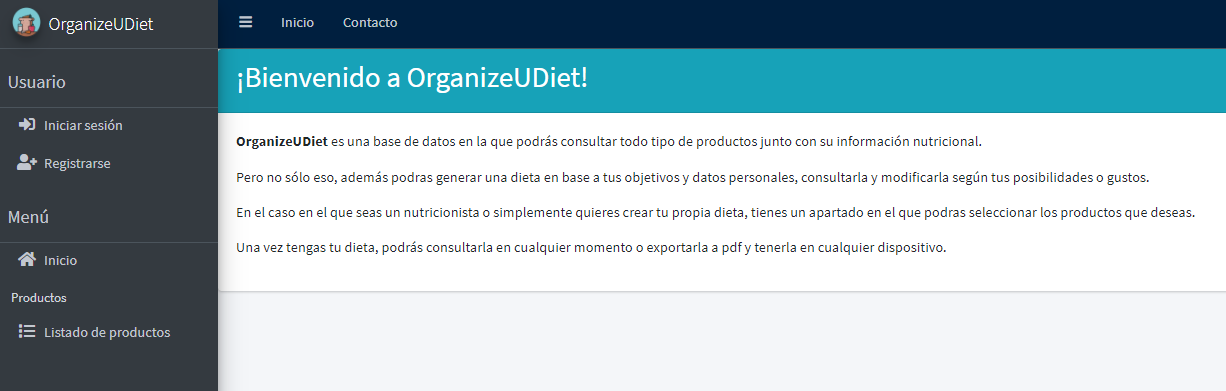
\includegraphics[scale=0.5]{index.png}}
  \caption{Página principal}
\end{figure}

\newpage
Podemos iniciar sesión si ya tenemos un usuario.

\begin{figure}[H]
  \centering
  \noindent\makebox[\textwidth]{
    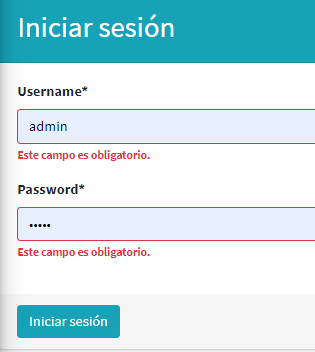
\includegraphics[scale=0.7]{login.png}}
  \caption{Vista login}
\end{figure}

\newpage
Registrarnos si no lo hemos hecho todavía.

\begin{figure}[H]
  \centering
  \noindent\makebox[\textwidth]{
    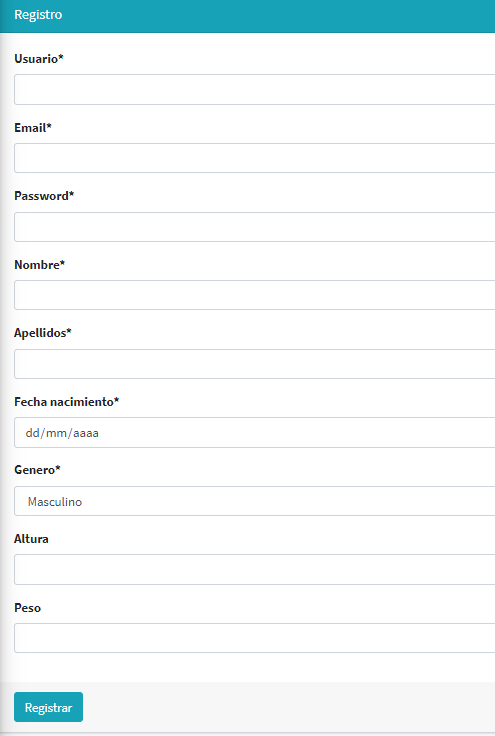
\includegraphics[scale=0.6]{registro.png}}
  \caption{Vista registro}
\end{figure}

\newpage
Podemos añadir productos, editarlos y borrarlos con un formulario con validación de datos.

\begin{figure}[H]
  \centering
  \noindent\makebox[\textwidth]{
    \includegraphics[scale=0.4]{añadirProducto.png}}
  \caption{Vista añadir producto}
\end{figure}

Visualizar el listado de productos, con enlace en el nombre para visualizarlo en detalle, con un paginador y un buscador.

\begin{figure}[H]
  \centering
  \noindent\makebox[\textwidth]{
    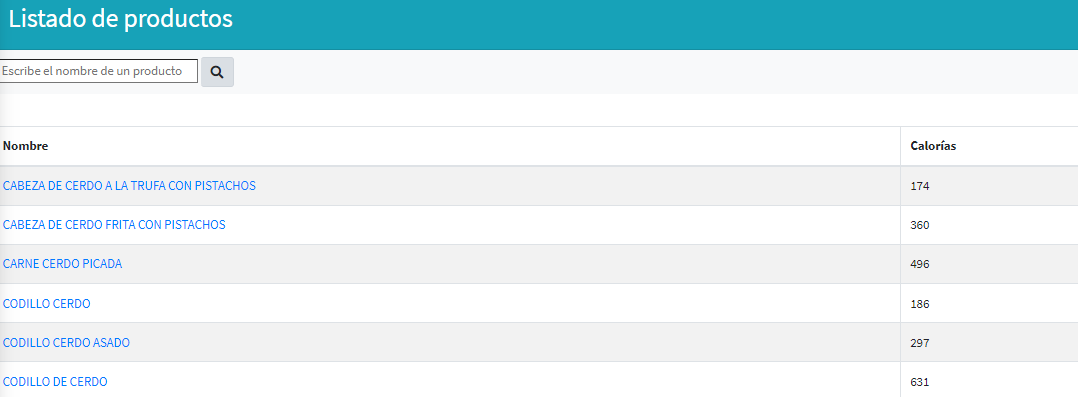
\includegraphics[scale=0.4]{listadoProductos.png}}
  \caption{Vista listado productos}
\end{figure}

Esta sería la vista de consultar los detalles de un producto.

\begin{figure}[H]
  \centering
  \noindent\makebox[\textwidth]{
    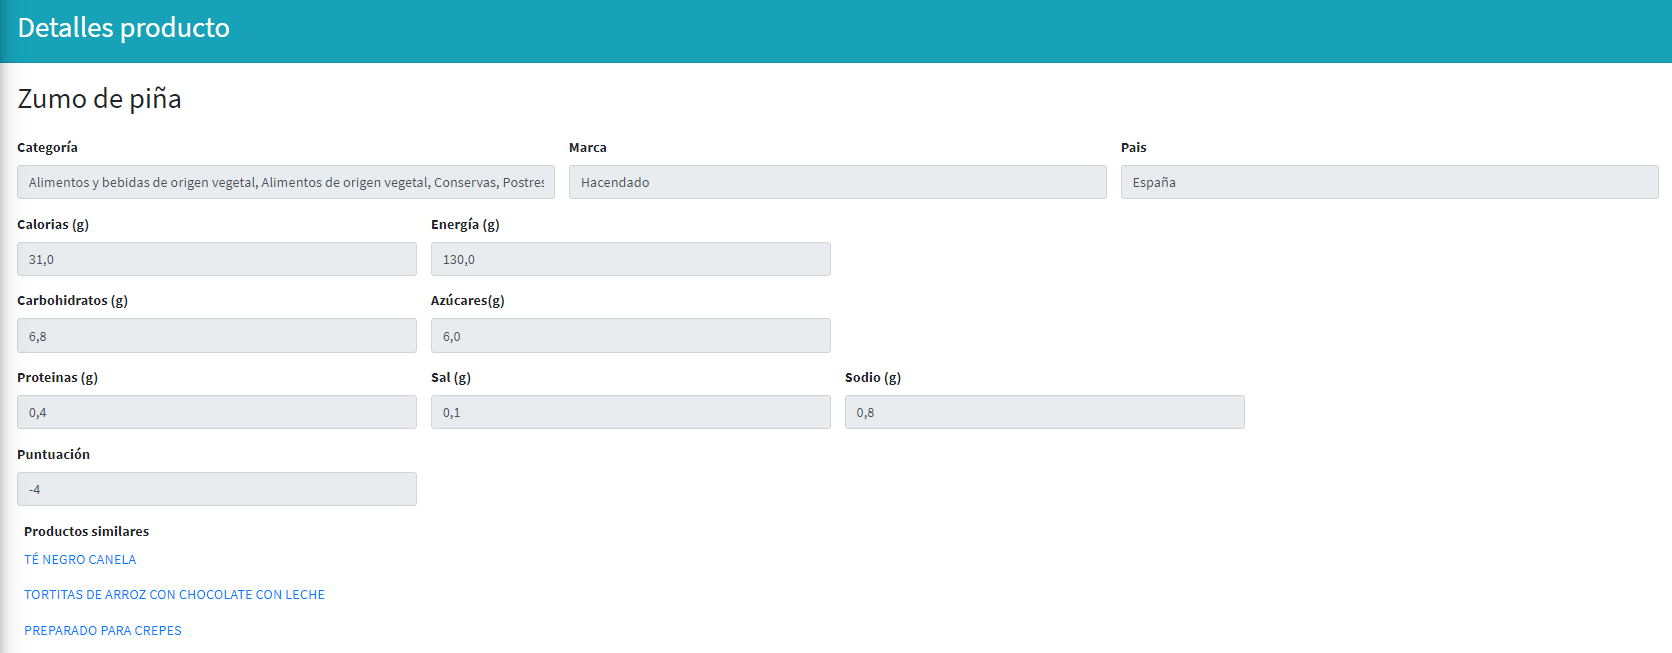
\includegraphics[scale=0.6]{consultarProducto.png}}
  \caption{Vista consultar producto}
\end{figure}

Tenemos la opción de visualizar productos similares.

\begin{figure}[H]
    \centering
    \noindent\makebox[\textwidth]{
      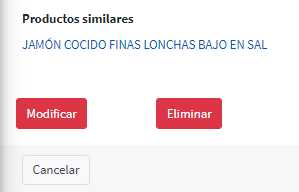
\includegraphics[scale=1]{productosSimilares.png}}
    \caption{Productos similares}
  \end{figure}

\newpage
Este sería el paginador.

\begin{figure}[H]
  \centering
  \noindent\makebox[\textwidth]{
    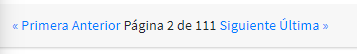
\includegraphics[scale=1]{paginador.png}}
  \caption{Paginador}
\end{figure}

Consultar nuestro perfil, modificarlo y eliminarlo.

\begin{figure}[H]
  \centering
  \noindent\makebox[\textwidth]{
    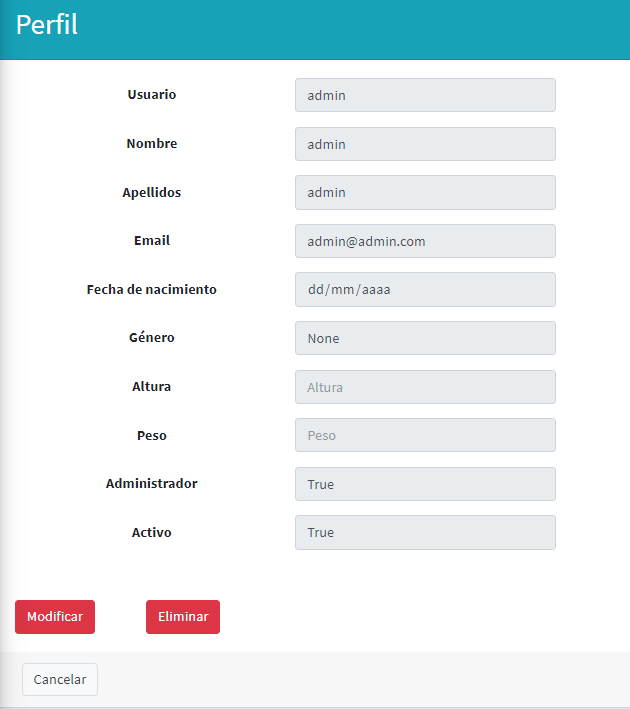
\includegraphics[scale=0.5]{consultarPerfil.png}}
  \caption{Vista consultar perfil}
\end{figure}

\newpage
Para la edición y borrado de objetos como pueden ser los productos, aparece un aviso para confirmar la acción.

\begin{figure}[H]
  \centering
  \noindent\makebox[\textwidth]{
    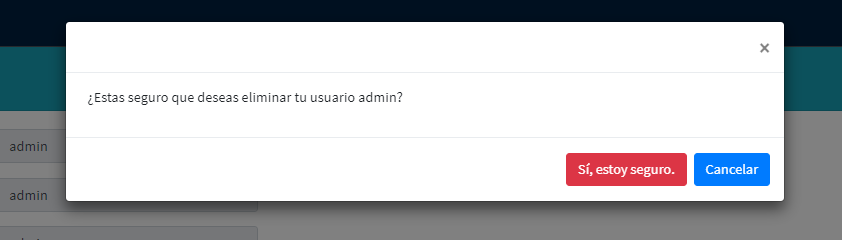
\includegraphics[scale=0.6]{modal.png}}
  \caption{Ejemplo de modal}
\end{figure}

Podemos crear una dieta seleccionando los productos que queramos y asignárnosla si somos un usuario o asignársela a otro usuario si somos un dietista.

\begin{figure}[H]
  \centering
  \noindent\makebox[\textwidth]{
    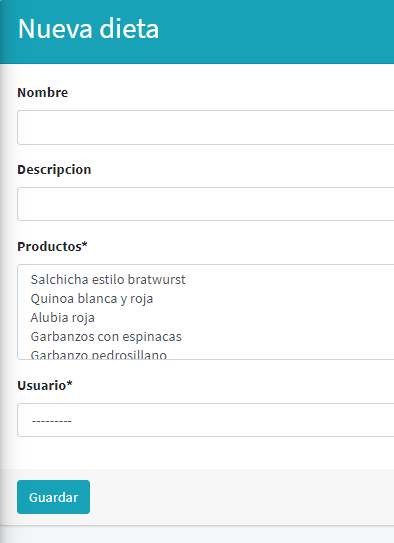
\includegraphics[scale=0.6]{crearDieta.png}}
  \caption{Vista crear dieta}
\end{figure}

\newpage
Este sería el formulario con el que obtendremos nuestra dieta.

\begin{figure}[H]
    \centering
    \noindent\makebox[\textwidth]{
      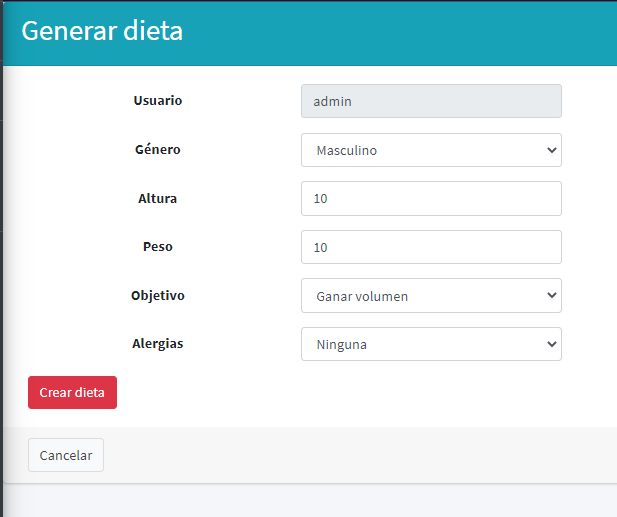
\includegraphics[scale=0.6]{generarDieta.png}}
    \caption{Formulario generar dieta}
  \end{figure}
  
Aquí podemos ver un listado con nuestras dietas, pudiendo visualizarla en detalle o exportarla a PDF.
  
  \begin{figure}[H]
    \centering
    \noindent\makebox[\textwidth]{
      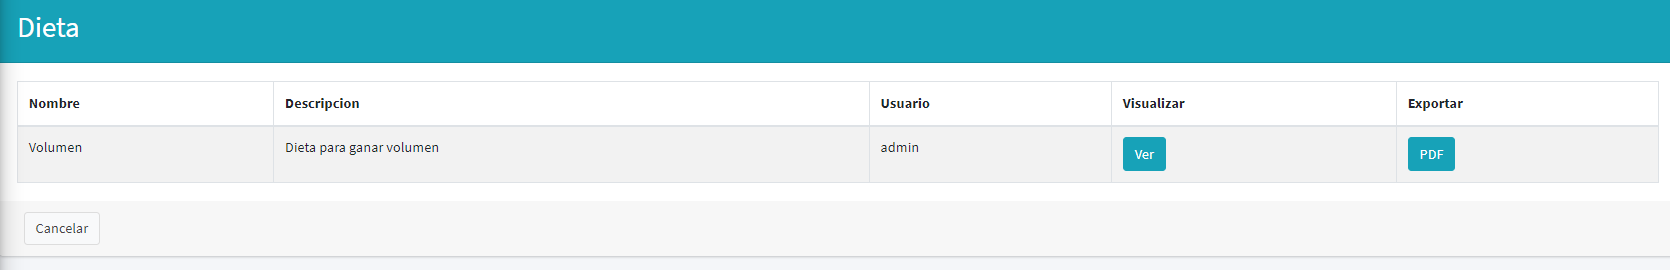
\includegraphics[scale=0.4]{mostrarDieta.png}}
    \caption{Vista mostrar dieta}
  \end{figure}

\newpage
Podemos visualizar los productos que contienen nuestra dieta.

\begin{figure}[H]
    \centering
    \noindent\makebox[\textwidth]{
      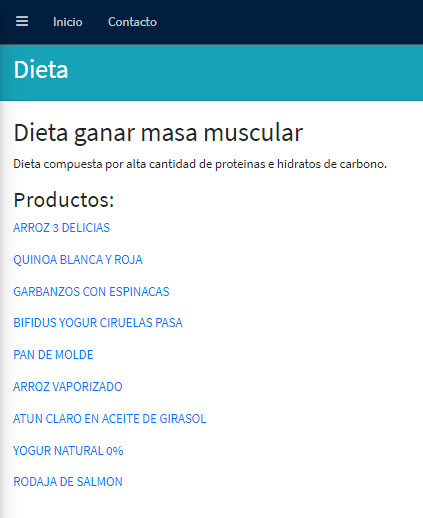
\includegraphics[scale=0.8]{verDieta.png}}
    \caption{Vista mostrar dieta}
  \end{figure}


